\section{Results}
\label{sec:results}

\subsection{Setup}

The corpus is a balanced subset of SONICS: 910 songs, 455 per class, real music
fetched from the source identifiers SONICS provides and generated music drawn
from its released archives. Clips are \SI{5}{\second}, four per song. After
decoding, 816 songs remained usable (361 real, 455 synthetic). The shortcut
diagnostic on this corpus reads 0.737 AUROC, below the threshold at which we
regard a detector score as interpretable.

\subsection{In-distribution}

On the held-out split ($n = 122$) the detector reaches $F_1$ 0.957, accuracy
0.951, AUROC 1.000 and expected calibration error $1.54\times10^{-4}$.
Validation $F_1$ reaches 1.000 at the first epoch and remains there, so this
figure is saturated and should be read as a ceiling rather than a measurement of
architectural quality (Section~\ref{sec:limitations}).

\subsection{What the architecture contributes}

The detector's novelty claim rests on the head: learned attention over all
thirteen MERT layers, and learned attention rather than averaging when pooling
frames and clips. Table~\ref{tab:ablation} replaces each of those choices in
turn, retraining from the same seed on the same split.

\begin{table}[t]
\centering
\caption{Pooling and layer ablations ($n = 122$, 55 real). Every variant is
retrained from the same seed. The three left-hand columns are identical to
every digit across the first three rows; the entire spread across all four
architectures is one song.}
\label{tab:ablation}
\begin{tabular}{lSSSS}
\toprule
Variant & {$F_1$} & {AUROC} & {FPR} & {ECE} \\
\midrule
Layer attention + attention pooling (full) & 0.9926 & 1.000 & 0.018 & 0.0041 \\
Mean frame pooling                         & 0.9926 & 1.000 & 0.018 & 0.0082 \\
Last hidden state only                     & 0.9926 & 1.000 & 0.018 & 0.0073 \\
Mean clip$\rightarrow$song pooling         & 1.0000 & 1.000 & 0.000 & 0.0001 \\
\bottomrule
\end{tabular}
\end{table}

The result is negative and we report it as such. Discarding twelve of the
thirteen hidden states changes nothing. Replacing attention over frames with an
unweighted mean changes nothing. Read as counts rather than rates, the first
three rows each classify 121 of 122 songs correctly and each make the same
single false positive out of 55 real songs; the fourth makes none. The full
range of the table is one song, which is not a difference any of these
architectures can be credited with.

Two things follow. The architectural contribution is not measurable on this
corpus, so the case for the design has to rest on the explanations it makes
available---which Section~\ref{sec:discussion} argues is where its value
actually lies---rather than on accuracy. And the one variant that is not
identical is mean clip-to-song pooling, which is nominally the \emph{best} row.
We draw no conclusion from that either: a single song separates it from the
rest, and the run is one seed.

What the table cannot do is discriminate, because validation $F_1$ reaches 1.000
at the first epoch for every variant (Section~\ref{sec:limitations}). A corpus
that separates this easily cannot rank heads. The honest reading is that this
experiment is not yet informative, not that the choices are equivalent in
general.

\subsection{Robustness}

Table~\ref{tab:robustness} reports degradation under six held-out perturbations,
none seen during training.

\begin{table}[t]
\centering
\caption{Robustness to held-out degradations ($n = 122$). AUROC is largely
preserved while $F_1$ falls, indicating that discrimination survives but the
operating point does not.}
\label{tab:robustness}
\begin{tabular}{llSS S}
\toprule
Condition & Family & {$F_1$} & {AUROC} & {$\Delta F_1$} \\
\midrule
Clean            & ---    & 0.957 & 1.000 & 0.000 \\
Time stretch     & time   & 0.912 & 1.000 & -0.046 \\
Reverb           & room   & 0.788 & 1.000 & -0.169 \\
Low-pass \SI{4}{\kilo\hertz} & filter & 0.775 & 0.989 & -0.183 \\
MP3 \SI{32}{\kilo\bit\per\second} & codec & 0.766 & 0.944 & -0.191 \\
Pitch shift      & pitch  & 0.724 & 0.999 & -0.233 \\
Additive noise   & noise  & 0.709 & 0.904 & -0.248 \\
\bottomrule
\end{tabular}
\end{table}

The pattern matters more than the magnitudes. Under four of six conditions AUROC
remains at or above 0.989 while $F_1$ falls by up to 0.233. The detector's
ability to rank synthetic above real audio is robust; the threshold at which
that ranking becomes a decision is not. A study reporting $F_1$ alone would
describe this as a robustness failure, when it is a calibration failure.

\begin{figure}[t]
\centering
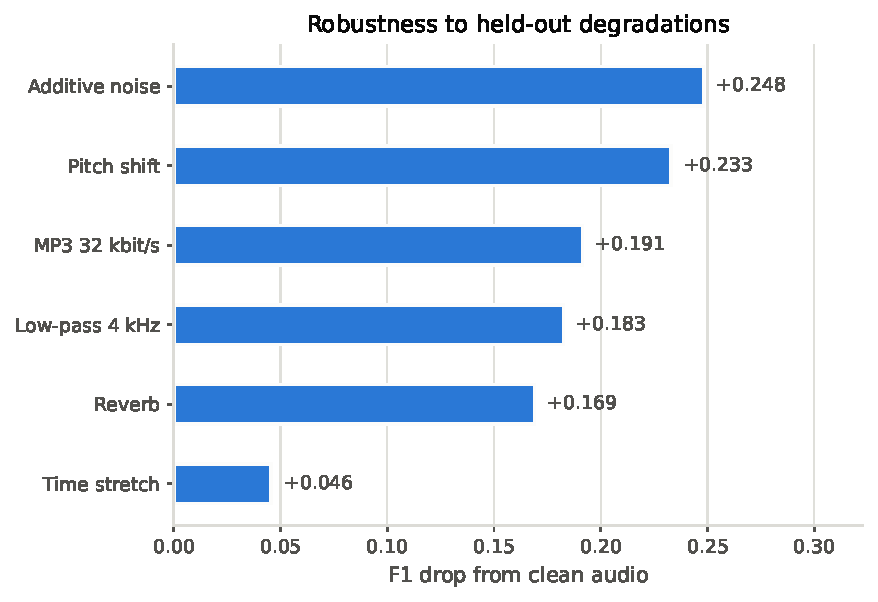
\includegraphics[width=\textwidth]{figures/fig_robustness.pdf}
\caption{$F_1$ loss under each held-out degradation, grouped by perturbation
family. No condition was seen during training. The ordering is not the one a
codec-artefact account of detection would predict: pitch shift and additive
noise cost more than \SI{32}{\kilo\bit\per\second} MP3.}
\label{fig:robustness}
\end{figure}

\subsection{Cross-generator with a shared corpus}

Table~\ref{tab:gensplit} reports both Suno/Udio directions. Each is trained on
one generator and tested on the other, with real songs divided disjointly and
both classes balanced in each half.

\begin{table}[t]
\centering
\caption{Cross-generator transfer within SONICS ($n = 362$ per direction). The
all-positive baseline is 0.667; both results are well clear of it.}
\label{tab:gensplit}
\begin{tabular}{lSSSSS}
\toprule
Direction & {In-dist. $F_1$} & {Cross $F_1$} & {Cross AUROC} & {FPR} & {ECE} \\
\midrule
Suno $\rightarrow$ Udio & 1.000 & 0.963 & 0.9995 & 0.000 & 0.031 \\
Udio $\rightarrow$ Suno & 1.000 & 0.977 & 1.0000 & 0.000 & 0.022 \\
\bottomrule
\end{tabular}
\end{table}

Degradation is $-0.037$ and $-0.023$ in $F_1$, against the $-0.361$ reported by
Cros Vila et al. False-positive rate is zero in both directions and calibration
error remains near 0.03. Withholding an entire generative family, with the real
class held fixed, costs the detector almost nothing.

\subsection{Cross-corpus}

Evaluated on FakeMusicCaps---five unseen text-to-music generators (AudioLDM2,
MusicGen, MusicLDM, Mustango, StableAudioOpen; 75 clips each) against 250
MusicCaps recordings---the same detector reaches AUROC 0.598, marginally above
chance, with ECE 0.365 and \textbf{FPR 1.00}. Per generator, AUROC ranges from
0.438 (AudioLDM2, below chance) through 0.512, 0.618 and 0.654 to 0.770
(Mustango).

The reported $F_1$ is 0.750. A classifier labelling every input synthetic scores
0.750 on this class balance. The detector has labelled every clip synthetic, and
the figure is the class ratio, not a result. Had we reported $F_1$ against the
published 0.629 baseline we would have claimed a $+0.121$ improvement for a
total failure.

\subsection{The two results together}

Figure~\ref{fig:transfer} places them side by side. Discrimination and
recognition-of-real-music move together and identify the mechanism: FPR 1.00
means every genuine MusicCaps recording was called synthetic. The detector did
not fail to recognise new generators; it failed to recognise new real music.

\begin{figure}[t]
\centering
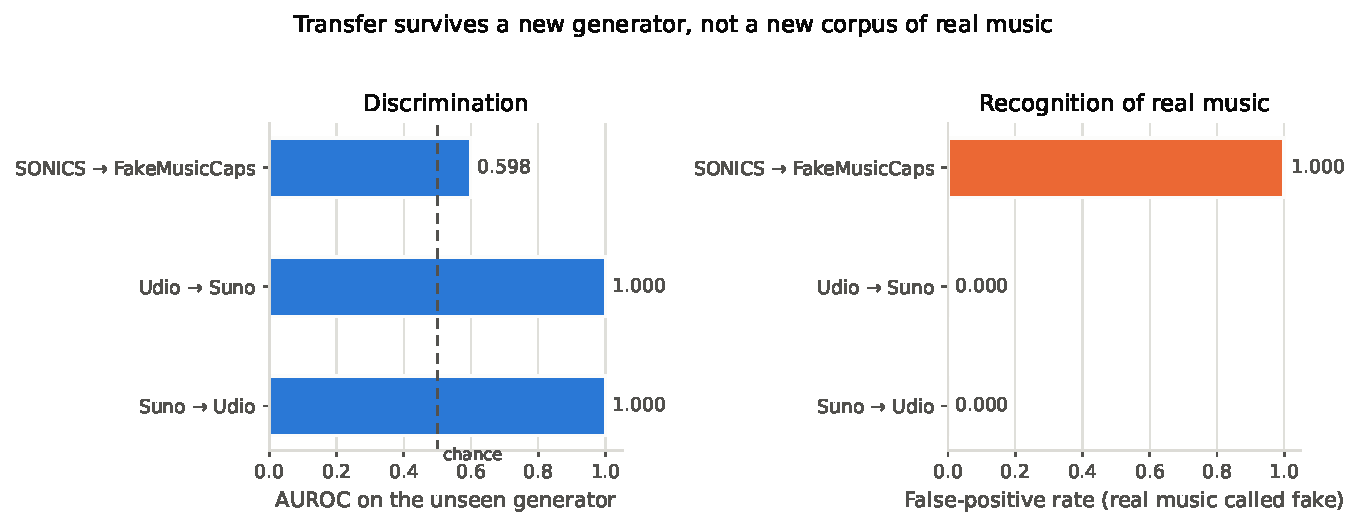
\includegraphics[width=\textwidth]{figures/fig_transfer.pdf}
\caption{Transfer survives a new generator but not a new corpus of real music.
Left: AUROC on the unseen generator. Right: the fraction of genuine recordings
labelled synthetic. With the real class held fixed (Suno/Udio) AUROC is $\geq
0.9995$ and FPR is zero; when the corpus of real music also changes
(FakeMusicCaps) AUROC falls to 0.598 and every real clip is misclassified.}
\label{fig:transfer}
\end{figure}

\subsection{Explanation faithfulness}

Across twelve explained songs, balanced by class, every explanation of a real
recording beat its random baseline (6/6, mean gap $-2.97$) and no explanation of
a generated recording did (0/6, mean gap $+1.31$). For synthetic audio, masking
the regions the explanation marks as important moves the logit \emph{less} than
masking at random. Figure~\ref{fig:faithfulness} shows the deletion curve for
one real recording, where the explanation-ordered curve stays below the random
one across the whole sweep.

\begin{figure}[t]
\centering
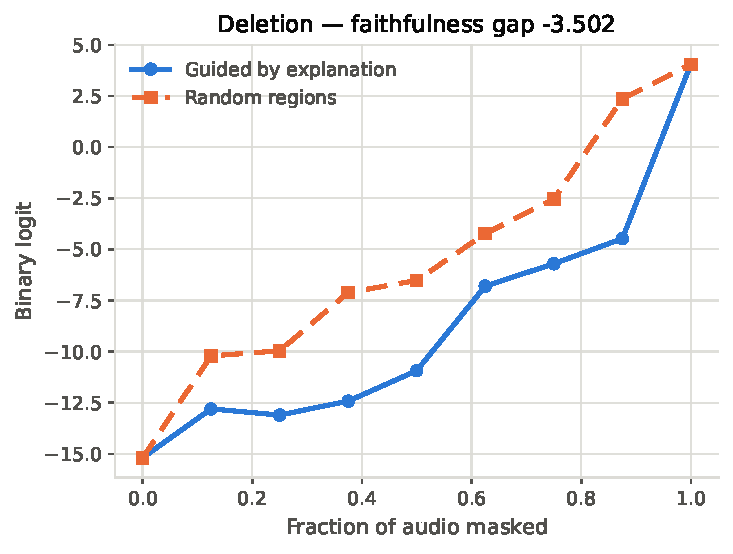
\includegraphics[width=0.78\textwidth]{figures/fig_faithfulness.pdf}
\caption{Deletion curve for a real recording (\texttt{real\_27619},
faithfulness gap $-3.50$). Audio is masked in order of attributed relevance
(solid) or at random (dashed) and the binary logit is re-measured. The
explanation is faithful when its curve sits below the random one, as it does
here across the whole sweep. Every real recording in the audit behaves this way;
no generated one does.}
\label{fig:faithfulness}
\end{figure}

Temporal attribution is therefore inadequate for exactly the class the
application cares about. The evidence a detector uses for ``synthetic'' is not
localised in time, which is consistent with frequency-domain accounts of
AI-music artefacts~\cite{afchar2025ismir} and is a direct argument for
frequency-resolved explanation over Grad-CAM-style temporal methods.

Layer attention converged to a near-uniform profile: weights run 0.073--0.080
about a uniform $1/13 = 0.077$, a spread of 1.09$\times$ between the largest and
smallest. Shapley attribution over the same thirteen layers runs 0.003--0.172, a
spread of 49$\times$, and its coefficient of variation is 20 times the
attention profile's (0.591 against 0.029)
(Figure~\ref{fig:layers}). Worse than uninformative, the two \emph{disagree}:
rank agreement between the attention profile and the Shapley attribution is
negative for every audited song, and strongly so for real recordings (mean
$-0.69$, against $-0.20$ for generated ones; overall $-0.45$). The layers the
model's own gate weights most highly are not the layers whose removal moves the
logit. Reporting Level~1 alone---the explanation the architecture supplies for
free, and the one most readily quoted---would have produced a confident
explanation that the model's behaviour contradicts.

\begin{figure}[t]
\centering
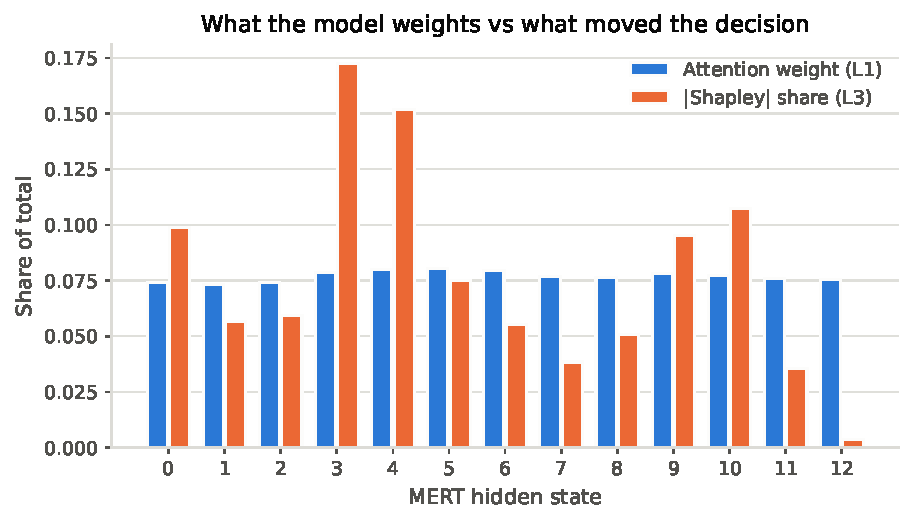
\includegraphics[width=\textwidth]{figures/fig_layers.pdf}
\caption{What the model says it weights against what actually moved the
decision, paired per MERT hidden state. Both quantities are normalised to sum to
one so that a single axis is meaningful. The attention weights (L1) are flat:
0.073--0.080 against a uniform $1/13 = 0.077$, a spread of 1.09$\times$. The
Shapley shares (L3) span 0.003--0.172, a spread of 49$\times$, and concentrate
in the middle of the stack (layers 3--4). The last hidden state, the one a
conventional last-layer probe would use, carries the smallest share of all.}
\label{fig:layers}
\end{figure}
